\section{Results and Discussion}
\label{Sec:Res}

In this section, we compare the proposed method on the three datasets with two categories of methods, including recent non-deep-learning algorithms, such as Minh-CNN\cite{IEEEexample:mnih2013machine}, Satio-multi~\cite{IEEEexample:saito2016multiple} and Context~\cite{IEEEexample:audebert2017deep}, and deep-learning based approaches, including FCN~\cite{IEEEexample:Long_2015_CVPR}, SegNet~\cite{IEEEexample:badrinarayanan2017segnet}, Deeplab~\cite{IEEEexample:chen2016deeplab} and U-Net~\cite{IEEEexample:ronneberger2015u}.


Moreover, for the HF-FCN itself, we expect to investigate which kind of information extracted from feature extractors and how the effects of extracted information on the final prediction.
Thus, some up-sampled feature maps ${\left\{U_k\right\}}$ are presented.
And several variants of HF-FCN which combine different up-sampling feature maps from Part 2 are proposed.
%
For dataset ${b)}$ and ${c)}$, multichannel information is provided.
Hence, to explore the impact of other information on the results, a simple experiment is presented which concatenate different kinds of information as input of HF-FCN.
In addition, different feature extractor networks are tried as our Part 1 network, including VGG16 Net and ResNet.
The results and discussion of above mentioned experiments are shown below.


\begin{figure}[t] 
\centering
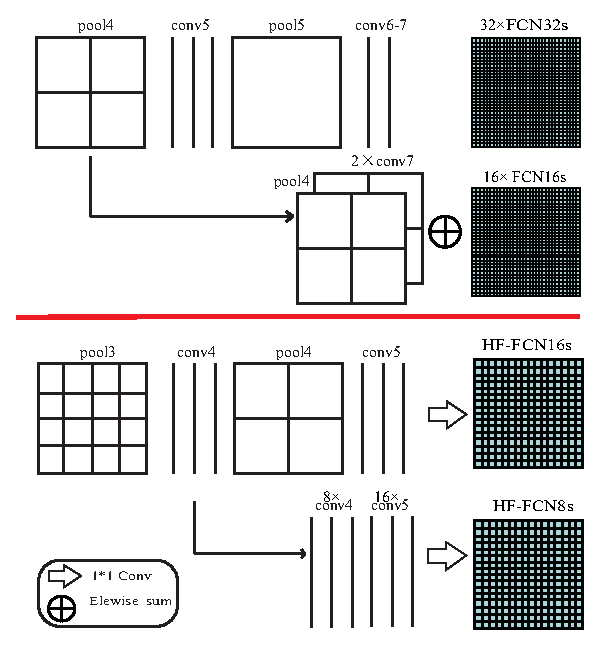
\includegraphics[width=7.8cm]{Figures/vairants.eps}
\caption{FCN and HF-FCN variants. The feature maps generated from final group are fused into a coarse result, which is HF-FCN16s. 
The variant called HF-FCN8s concatenates the feature maps from the last 2 groups with the same fusion operation, and so on.}
\label{fig:Variants}
\end{figure}

\subsection{Massachusetts Dataset}
On the Massachusetts dataset, both the non-deep-learning algorithms and deep-learning based approaches are compared with our method. 
Table~\ref{table:Mass-results} presents the quantitative analysis results with the standard and relaxed precisions, and recall as our evaluation criteria.
%The best results of our methods and others' methods are marked in bold. 
Our method shows obvious superiority in terms of speed and precision. 
%
Compared with Satio-multi-MA\&CIS~\cite{IEEEexample:saito2016multiple}, the best among the non-deep-learning algorithms, the VGG version of our HF-FCN achieves $5.5\%$ and $1.3\%$ higher standard and relaxed recall.
%
Meanwhile, our HF-FCN reduces the time cost from 67.84s to 1.07s, and gets a $63\times$ speedup.
These significant improvements demonstrate that HF-FCN achieves better performance in both effectiveness and efficiency.

While comparing our HF-FCN with recent semantic segmentation methods, as shown in Table~\ref{table:Mass-results} and Fig.~\ref{fig:Mass-visi-result}, we get about $3\times$ speedup without sacrificing the accuracy, compared with the most state-of-the art method U-Net~\cite{IEEEexample:ronneberger2015u}.
From the visual results, our method preserves the details and integrity of the building better than others.
\begin{table}
\vspace{-0.2cm}
\setlength{\belowcaptionskip}{-1cm} 
\centering
\caption {Correctness at breakeven of HF-FCN v.s. \cite{IEEEexample:mnih2013machine}\cite{IEEEexample:saito2016multiple}\cite{IEEEexample:alshehhi2017simultaneous}\cite{IEEEexample:Long_2015_CVPR}\cite{IEEEexample:badrinarayanan2017segnet}
\cite{IEEEexample:ronneberger2015u}\cite{IEEEexample:chen2016deeplab}on Massachusetts test set. Cost time is computed in the same computer with a single NVIDIA Titan 12GB GPU}
\label{table:Mass-results}
\begin{tabular}{cccc}
\hline
&Recall ($\rho$ = 3)&Recall ($\rho$ = 0)&Time (s)\\
\hline
Mnih-CNN \cite{IEEEexample:mnih2013machine}&0.9271&0.7661&8.70\\
Mnih-CNN+CRF\cite{IEEEexample:mnih2013machine} &0.9282&0.7638&26.60\\
Satio-multi-MA \cite{IEEEexample:saito2016multiple}&0.9503&0.7873&67.72\\
Satio-multi-MA\&CIS \cite{IEEEexample:saito2016multiple}&0.9509&0.7872&67.84\\
Alshehhi-GAP+seg \cite{IEEEexample:alshehhi2017simultaneous}&0.955&{--}&{--} \\ \hline
FCN\_4s\cite{IEEEexample:Long_2015_CVPR}&0.839&0.6147&4.20\\
SegNet\cite{IEEEexample:badrinarayanan2017segnet}&0.7710&0.5675&2.39\\
U-Net\cite{IEEEexample:ronneberger2015u}& $\bm{0.9638}$& $\bm{0.8357}$& 3.165\\
DeepLab\_V2\cite{IEEEexample:chen2016deeplab}&0.9620&0.7575&$\bm{1.89}$\\ \hline
HF-FCN(VGG16 Net)&0.9643& $\bm{0.8424}$ &1.07\\
HF-FCN(VGG+data aug)&$\bm{0.9650}$&0.8357&1.38\\
HF-FCN(ResNet)&0.9588&0.8175&2.42\\
HF-FCN16s &0.9330&0.7233&0.85\\
HF-FCN8s &0.9643&0.8171&0.93\\
HF-FCN4s &0.9632&0.8394&$\bm{0.99}$\\
\hline
\end{tabular}
\end{table}

In addition, to explore which kinds of information extracted by hierarchical fusion operation in Part 2.
Some upsampled feature maps ${\left\{U_1,U_2,U_3,U_7,U_{10},U_{13}\right\}}$ are shown in Fig.~\ref{fig:feature_maps}.
The U1\_1 (${U_1}$) in Fig.~\ref{fig:feature_maps}(b) means the upsampled feature map from F1\_1 (${F_1}$) which are feature maps generated from conv1\_1 in VGG16 Net.
Due to small receptive field of conv1\_1 and conv1\_2, they extract low-level features like edges.
And the U1\_2 (${U_2}$) looks like an over-segmentation which groups pixels with similar color or texture into a subregion.
With the deepening of the network, in the U2\_1 (${U_3}$), as Fig.~\ref{fig:feature_maps}(d) shows, shape information is augmented.
And from the U3\_3 (${U_7}$), we can see that regions with significantly varying appearance are merged into an integrated building by considering high-level features.
In U4\_3 (${U_{10}}$) and U5\_3 ($U_{13}$), more semantic information of rooftop is got, which can distinguish the rooftop and the roads with similar color and deal with the problem caused by shadow.
The final prediction results are shown in Fig.~\ref{fig:feature_maps}(h).

Secondly, to explore the effects of the feature maps generated from each feature extract stage ${\left\{F_k\right\}}$ on the final result, variants of HF-FCN which are counterpart of FCN are designed.
Fig.~\ref{fig:Variants} shows the contrast diagram of variants of FCN and HF-FCN.
Unlike FCN, a fusion operation rather than summation are leveraged to build our HF-FCN 16s, 8s and 4s.
The precision-recall(PR) curves, prediction results and quantitative results of HF-FCN variants are shown in Fig.~\ref{fig:Mass-variants-PR}, Fig.~\ref{fig:Mass-variants-visi} and Table~\ref{table:Mass-results} respectively. \cxj{Figure 8, Figure 9 and Table \Rmnum{5}}.
From the disgrams, we can get the following conclusions easily:
\begin{itemize}
 \item The prediction result obtained from the last layer gets a coarse result, which loses much of location information that are mainly encoded in the shallow feature maps. 
 \item The largest gap presented between HF-FCN16s and HF-FCN8s about 9{\%} in recall rates, it may suggest that the most information supplement to the HF-FCN is got in middle layers.
 \item The PR curves of HF-FCN4s and HF-FCN almost coincide. It illustrates the low-level information has little effect on the prediction results.
 \item with the addition of the shallow feature map, the network is more distinct for the segmentation of tiny buildings, which solves the problem of easy adhesion to adjacent buildings.
\end{itemize}
Since, all the feature maps contained useful hierarchical information that is critical to the final prediction.

\begin{figure}  
\begin{center}
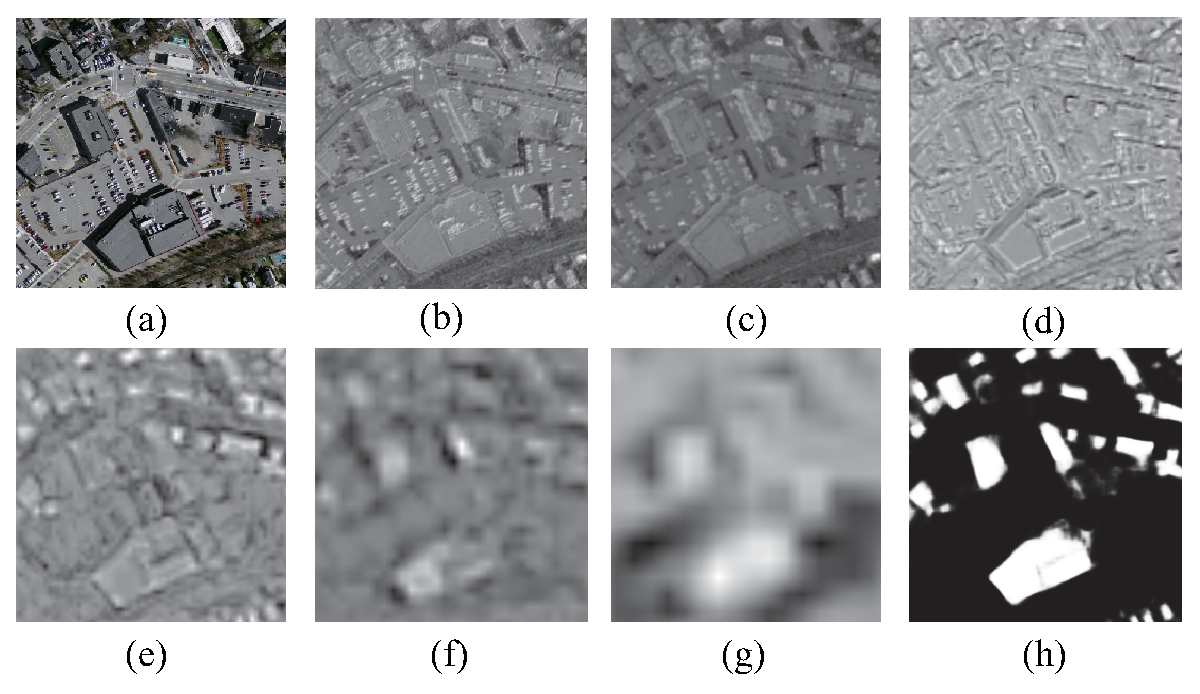
\includegraphics[width=8.7cm]{Figures/feature_maps.eps}
\caption{(a) Input aerial image. (b-g) Feature maps of U1\_1, U1\_2, U2\_2, U3\_3, U4\_3, U5\_3, respectively. (h) Predicted label map. All the images are normalized to the range of ${0-255}$.}
\label{fig:feature_maps}
\end{center}
\end{figure}


In the end, we want to prove that our fusion operations learn the connections between feature maps. The connection weights of F1\_1, F4\_1 and Part 3 are shown in Fig.~\ref{fig:Mass-weights}.
The weights are not the same, which means that fusion operations have effect on feature combination.
From the Fig.~\ref{fig:Mass-weights} (a) to Fig.~\ref{fig:Mass-weights} (c), the range of weights increases gradually. 
And from the Fig.~\ref{fig:Mass-weights} (c), we can arrive at the conclusion that the different layers have virous effects on the final result.
For example, the U1\_1 has little effect on the prediction while the U3\_2 and U4\_3 play more important roles on the final prediction.
It also in accordance with our experimental results that middle layers provide more information.
\cxj{Weight for what? to fuse feature map? The distribution does not make too much sense. }

\begin{figure}
\vspace{-0.2cm}
\setlength{\abovecaptionskip}{-0cm}
\setlength{\belowcaptionskip}{-2cm}  
\centering
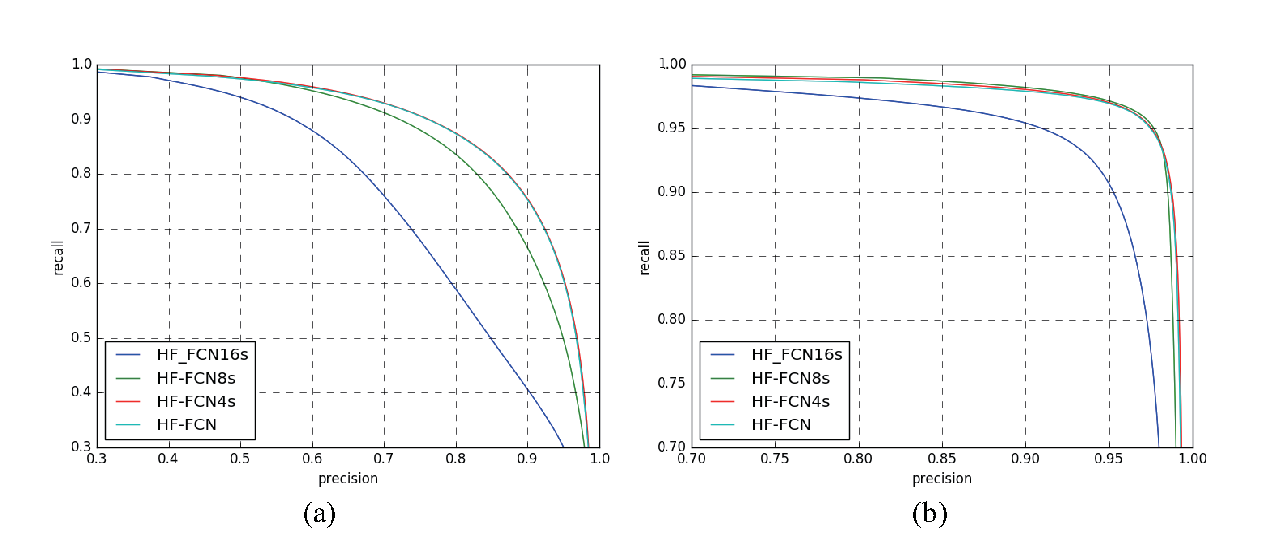
\includegraphics[width=8.7cm]{Figures/HF-FCN-variant-PR.eps}
\caption{The relaxed PR curves from HF-FCN variants with two slack parameters. The slack parameter $\rho$ on the left is 0. And $\rho$ = 3 on the right.}
\label{fig:Mass-variants-PR}
\end{figure}

\begin{figure}
\vspace{-0cm}
\setlength{\abovecaptionskip}{-0cm}  
\setlength{\belowcaptionskip}{-1cm}  
\centering
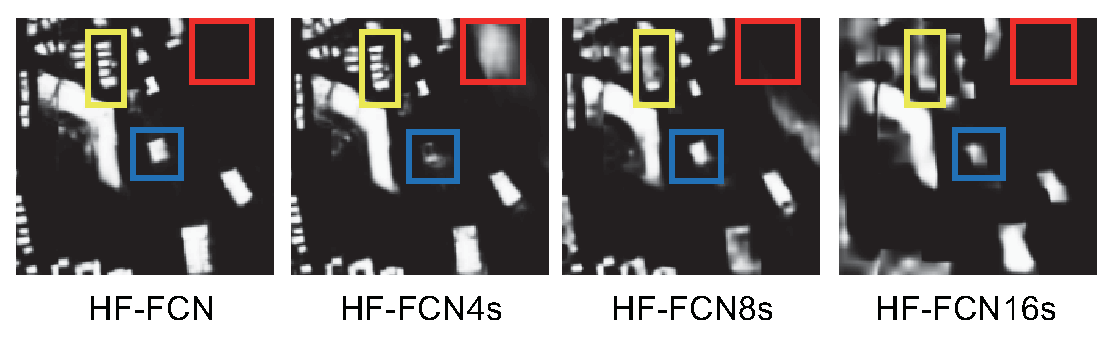
\includegraphics[width=8.7cm]{Figures/HF-FCN_variants_result.eps}
\caption{Prediction results of HF-FCN, HF-FCN4s, HF-FCN8s and HF-FCN16s. The yellow box shows the continuous refinement of the tiny buildings. The red and blue boxes show the mutual promotion and contradiction between different layers.}
\label{fig:Mass-variants-visi}
\end{figure}

\begin{figure*}
\vspace{-0.5cm}
\setlength{\abovecaptionskip}{-0cm}
\setlength{\belowcaptionskip}{-1cm}  
\centering
\includegraphics[width=17cm,height = 7cm]{Figures/mass_visi_result.eps}
\caption{From left to right: (a) input images, results of (b) Mnih-CNN+CRF, (c) Satio\-multi\-MA\&CIS, (d) FCN4s, (e) SegNet, (f) DeepLab\_V2, (g) U-Net, and (h) Our HF-FCN. We show the true positives in green, false positives in blue, and false negatives in red.}
\label{fig:Mass-visi-result}
\end{figure*}

\begin{figure}
\vspace{-0.4cm}
\setlength{\abovecaptionskip}{-0cm}
\setlength{\belowcaptionskip}{-1cm}  
\centering
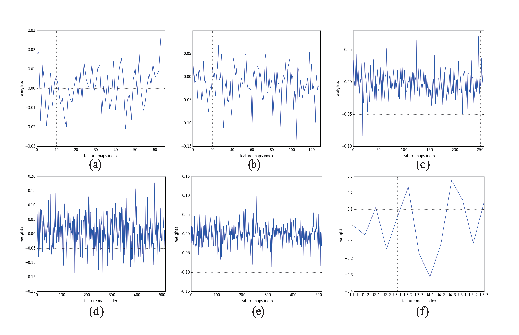
\includegraphics[width=9cm]{Figures/weights.eps}
\caption{(a) is weights learned by F1\_1, (b) is weights learned by F4\_1, (c) is weights learned by Part 3.}
\label{fig:Mass-weights}
\end{figure}

\subsection{Vaihingen dataset}
On Vaihingen dataset, three experiments are undertaken to explore the effects of different inputs, diverse variants and various methods. Three kinds of combinations of image channels are utilized as inputs. The inputs of the 3 channels are IR, R, G and adding the nDSM(normalized Digital Surface Model) as the forth channel. Based on it, DSM is added and made up 5-channel input. Three standards are used to make a more comprehensive evaluation. The evaluation results are shown in Table~\ref{table:vaihigen-3-4-5in-comp}, which illustrate that 3-channel input performed better than the others.
The Rec and Pre in Table~\ref{table:vaihigen-3-4-5in-comp} means the recall and precision of prediction results. And F1 indicates the F1 score of results.
The number in bold shows the best results of our methods and other methods. 
Visual results of our methods with different kinds of input are shown in Fig.~\ref{fig:Vaihingen-3-4-5in}.

\cxj{Do you compare with others?}


\begin{table}[htbp]
\caption {Performance comparison of the results of different inputs and methods on Vaihigen data set. \cxj{What are the numbers in the Img column?}}
\label{table:vaihigen-3-4-5in-comp}
\centering
\begin{tabular}{p{0.5cm}<{\centering}|p{1.1cm}<{\centering}|p{1.1cm}<{\centering}|p{1.1cm}<{\centering}|p{1.1cm}<{\centering}}
\hline
%&\multirow{2}{*}{Img}&\multicolumn{3}{c}{3\_in: IR, R, G} &\multicolumn{3}{|c|}{4\_in: IR, R, G, nDSM}&\multicolumn{3}{c}{5\_in: IR, R, G, DSM, nDSM}\\
&&Pre&Rec&F1\\
\hline
\multirow{2}{*}{Val}&3\_in&0.939&0.894&$\bm{0.915}$\\
&4\_in&0.96&0.865&0.909\\
&5\_in&0.939&0.880&0.907\\
\hline
\multirow{2}{*}{Test}&3\_in&$\bm{0.919}$&$\bm{0.930}$&$\bm{0.925}$\\
&4\_in&0.907&0.872&0.888\\
&5\_in&0.858&0.900&0.878\\
\hline\hline
\multicolumn{2}{c|}{FCN\_4s\cite{IEEEexample:Long_2015_CVPR}}&{0.871}&$\bm{0.884}$&{0.878}\\
\multicolumn{2}{c|}{SegNet\cite{IEEEexample:badrinarayanan2017segnet}}&{0.917}&{0.861}&{0.887}\\
\multicolumn{2}{c|}{U-Net\cite{IEEEexample:ronneberger2015u}}&{0.848}&{0.737}&{0.789}\\
\multicolumn{2}{c|}{DeepLab\_V2\cite{IEEEexample:chen2016deeplab}}&$\bm{0.926}$&{0.881}&$\bm{0.903}$\\
\hline \hline
\multicolumn{2}{c|}{HF-FCN16s}&{0.886}&{0.854}&{0.870}\\
\multicolumn{2}{c|}{HF-FCN8s}&{0.911}&{0.864}&{0.887}\\
\multicolumn{2}{c|}{HF-FCN4s}&{0.910}&{0.861}&{0.885}\\
\hline
\end{tabular}
\end{table}

Many experiments are done to compare with other methods, including methods using the same dataset and the other deep learning based methods. 
The detail comparison results using the same dataset are shown in Fig.~\ref{fig:Vaihingen-compared-others}. 
From a visual perspective, our method gets a much more refined roof region, both on continuity of labels and integrity of structural. 
The quantitative results of deep learning methods are shown in Table~\ref{table:vaihigen-3-4-5in-comp}. 
Compared to DeepLab\_V2\cite{IEEEexample:chen2016deeplab}, the F1 score of our method improves 2.2{\%}.

The results of diverse variants are shown in Fig.~\ref{fig:Vaihingen-variants}. The HF-FCN\_1 in Fig.~\ref{fig:Vaihingen-variants} indicates that the last conv layer in Part 3 does not use the previous trained model to initialize. And HF-FCN means that the whole layers use the pre-trained model to initialize. From the curves, the performance of HF-FCN exceeds the variants and gets a excellent result. Additionally, using the pre-trained weights of Part 3 has a significance in the final results.

\begin{figure}
\vspace{-0.2cm}
\setlength{\abovecaptionskip}{-0cm}
\setlength{\belowcaptionskip}{-1cm}  
\centering
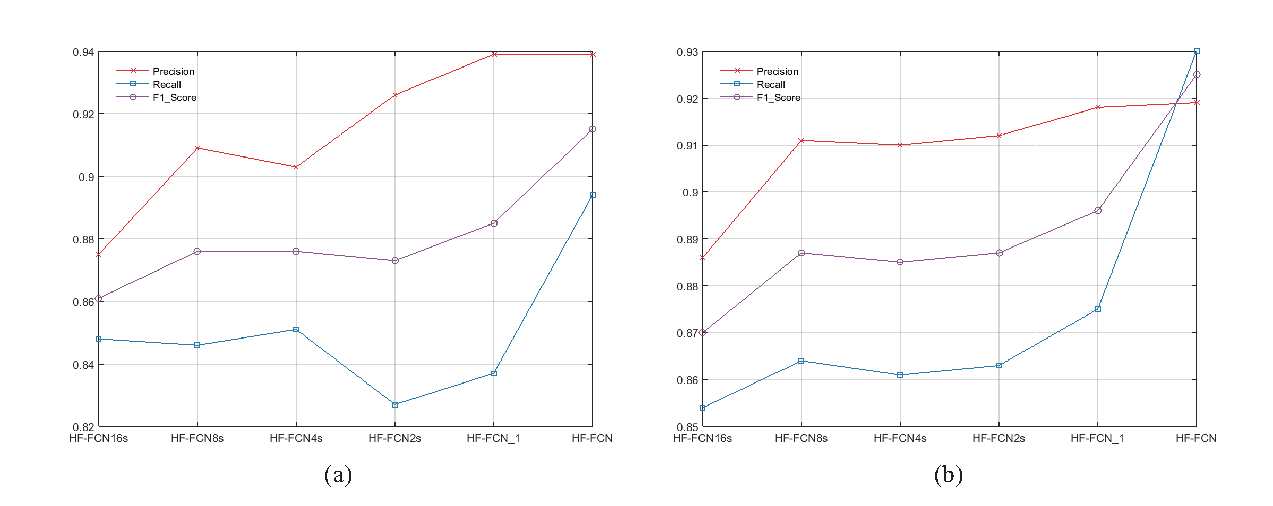
\includegraphics[width=8.7cm]{Figures/vaihingen_variants.eps}
\caption{Results of HF-FCN variants on Vaihingen dataset. (a) (b) shows the precision, recall and F1 score of validation set and test set of Vaihingen dataset respectively.\cxj{Bigger font}}
\label{fig:Vaihingen-variants}
\end{figure}

\begin{figure}
\vspace{-0.4cm}
\setlength{\abovecaptionskip}{-0cm}
\setlength{\belowcaptionskip}{-2cm}  
\centering
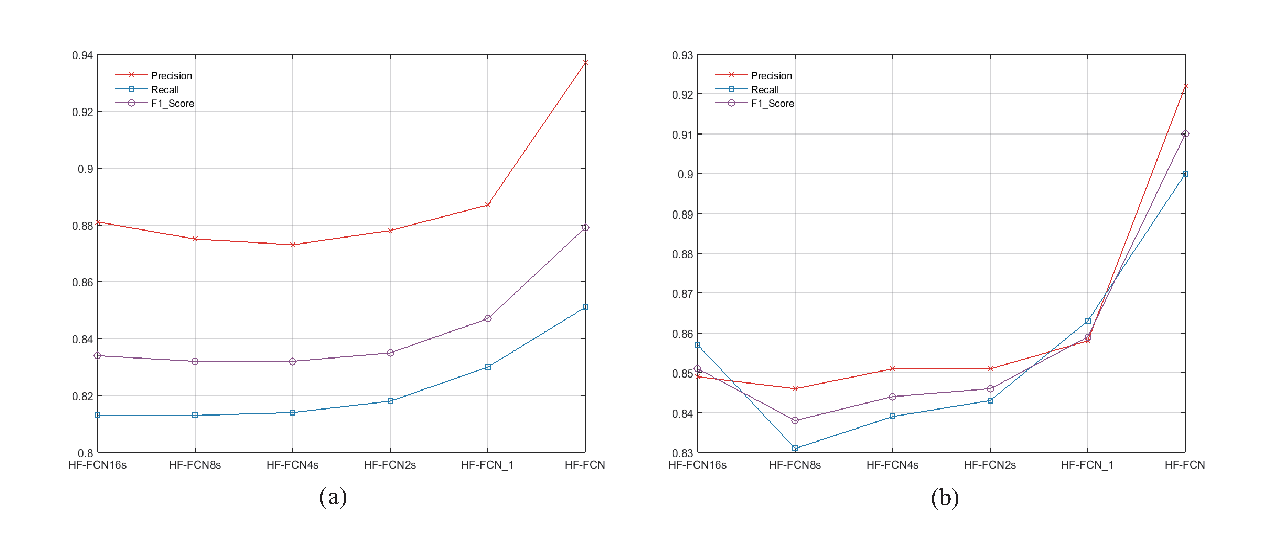
\includegraphics[width=8.7cm]{Figures/Potsdam_variants.eps}
\caption{Results of HF-FCN variants on Potsdam dataset. (a) (b) shows the precision, recall and F1 score of validation set and test set of Potsdam dataset respectively.}
\label{fig:Potsdam-variants}
\end{figure}

\begin{figure}
\vspace{-0.45cm}
\setlength{\abovecaptionskip}{-0cm}
\setlength{\belowcaptionskip}{-2cm}  
\centering
\includegraphics[width=8.7cm]{Figures/Vaihingen3_4_5in.eps}
\caption{Prediction results on Vaihingen dataset. (a) (b) (c) shows results of the 3-channel input, 4-channel input and 5-channel input of Vaihingen dataset respectively. Here, TP are shown in green, FP are shown in blue and FN are in red.}
\label{fig:Vaihingen-3-4-5in}
\end{figure}

\begin{figure}
\setlength{\abovecaptionskip}{-0cm}
\setlength{\belowcaptionskip}{-1cm}  
\centering
\includegraphics[width=8.7cm]{Figures/Vaihingen_compared_results.eps}
\caption{Results of different methods. (a) is input image, (b)(d)(g) are results of \cite{IEEEexample:audebert2017deep}, (c) is result of \cite{IEEEexample:marmanis2016semantic}, (f) is result of \cite{IEEEexample:unknown}, (g) is our result. The blue and yellow frames show some details between these methods.}
\label{fig:Vaihingen-compared-others}
\end{figure}

\subsection{Potsdam dataset}
 The same experiments are implemented on Potsdam dataset, including effects of different channels of input, comparing with other methods and results of diverse variants of HF-FCN. Firstly, we utilize nDSM and IR information as extra inputs based on the RGB input. The specific quantitative evaluation and intuitive visual prediction results are shown in Table~\ref{table:Potsdam-3-4-5in-comp} and Fig.~\ref{fig:Potsdam-3-4-5in-visi}. In the validation process, the 4-channel input including RGB, nDSM gets better overall performance. Meanwhile, the 5-channel input including RGB, nDSM and IR seems perform better in the course of testing. From the visual results, the 5-channel input network gets lower error detection rate which is shown on the image with small blue areas. And from the 3-channel input to 5-channel input, the F1 score increases from 0.879 to 0.891 on the validation set and increases 0.031 on the test set. It indicate that the other information of geographical feature have a certain effect on the final result.

 We compare HF-FCN with other methods using the Potsdam dataset and several deep learning methods. Some qualitative results of methods using Potsdam datast are shown in Fig.~\ref{fig:Potsdam-compared-others}.
 From the figure, we can easily see that HF-FCN got more remarkable segmentation results. And edges and structure of buildings are preserved better. The results of deep learning methods are shown in Table~\ref{table:Potsdam-3-4-5in-comp}. From the Table, the HF-FCN achieves the best result. And the F1 score far higher than the others.  

 As done on Vaihingen dataset, contrast experiments of HF-FCN variants are implemented. The performance curve of HF-FCN variants are shown in Fig.~\ref{fig:Potsdam-variants}.
 The HF-FCN\_1 in Fig.~\ref{fig:Potsdam-variants} indicates that the last conv layer in Part 3 does not use the previous trained model to initialize. And HF-FCN means that the whole layers use the pre-trained model to initialize. Initialization of parameters has a greater promotion on the final results.

\begin{table}[htbp]
\vspace{-0.2cm} 
\caption {Performance comparison of the results of different inputs and methods on Potsdam data set}
\label{table:Potsdam-3-4-5in-comp}
\centering
\begin{tabular}{p{0.5cm}<{\centering}|p{1.1cm}<{\centering}|p{1.1cm}<{\centering}|p{1.1cm}<{\centering}|p{1.1cm}<{\centering}}
\hline
%&\multirow{2}{*}{Img}&\multicolumn{3}{c}{3\_in: IR, R, G} &\multicolumn{3}{|c|}{4\_in: IR, R, G, nDSM}&\multicolumn{3}{c}{5\_in: IR, R, G, DSM, nDSM}\\
&&Pre&Rec&F1\\
\hline
\multirow{2}{*}{Val}&3\_in&0.937&0.851&0.879\\
&4\_in&0.937&$\bm{0.872}$&$\bm{0.894}$\\
&5\_in&$\bm{0.944}$&0.864&0.891\\
\hline
\multirow{2}{*}{Test}&3\_in&0.922&0.900&0.910\\
&4\_in&0.937&0.935&0.936\\
&5\_in&$\bm{0.940}$&$\bm{0.943}$&$\bm{0.941}$\\
\hline\hline
\multicolumn{2}{c|}{FCN\_4s\cite{IEEEexample:Long_2015_CVPR}}&{0.827}&{0.774}&{0.796}\\
\multicolumn{2}{c|}{SegNet\cite{IEEEexample:badrinarayanan2017segnet}}&{0.648}&{0.773}&{0.687}\\
\multicolumn{2}{c|}{U-Net\cite{IEEEexample:ronneberger2015u}}&$\bm{0.924}$&{0.705}&{0.799}\\
\multicolumn{2}{c|}{DeepLab\_V2\cite{IEEEexample:chen2016deeplab}}&{0.901}&$\bm{0.876}$&$\bm{0.887}$\\
\hline \hline
\multicolumn{2}{c|}{HF-FCN16s}&{0.849}&{0.857}&{0.851}\\
\multicolumn{2}{c|}{HF-FCN8s}&{0.846}&{0.831}&{0.838}\\
\multicolumn{2}{c|}{HF-FCN4s}&{0.851}&{0.839}&{0.844}\\
\hline
\end{tabular}
\end{table}

\begin{figure}
\vspace{-0cm} 
\setlength{\abovecaptionskip}{-0cm}
\setlength{\belowcaptionskip}{-2cm}  
\centering
\includegraphics[width=8.7cm]{Figures/Potsdam3_4_5in.eps}
\caption{Prediction results on potsdam dataset. (a) (b) (c) shows results of the 3-channel input, 4-channel input and 5-channel input of Vaihingen dataset respectively. Here, TP are shown in green, FP are shown in blue and FN are in red.}
\label{fig:Potsdam-3-4-5in-visi}
\end{figure}

\begin{figure}
\vspace{-0.2cm}
\centering
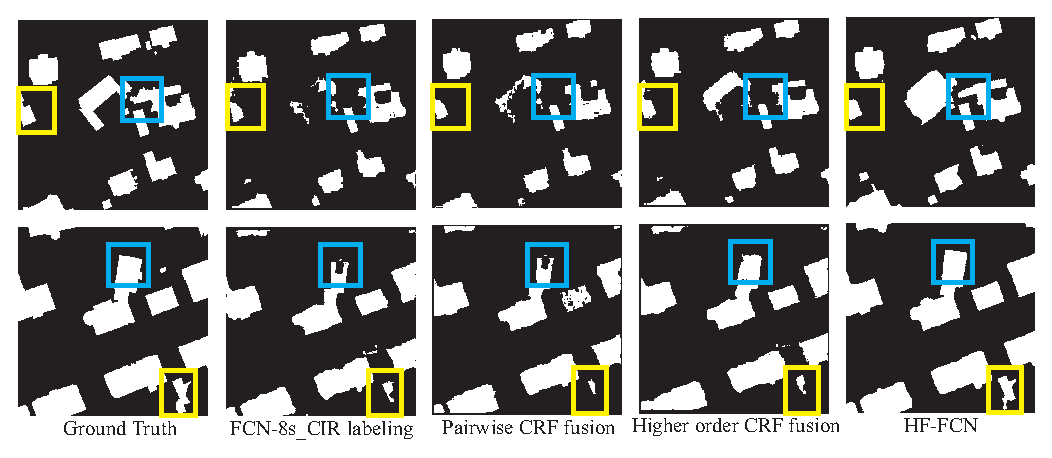
\includegraphics[width=8.7cm]{Figures/Potsdam_compared_results.eps}
\caption{Results of different methods. The second column is the results of using only the FCN with CIR(color-infrared image). Pairwise CRF fusion shows the result of fusing FCN-8s\_CIR with LiDAR data in a pairwise CRF. The results of using higher-order CRF\cite{IEEEexample:liu2017dense} as post processing are shown in third column. The last colunm shows our results.}
\label{fig:Potsdam-compared-others}
\end{figure}
